%%%%%%%%%%%%%%%%%%%%%%%%%%%%%%%%%%%%%%%%%%%%%%%%%%%%%%%%%%%%%%%%%%%%%%%%%%%%%%%%%%%%%%%%%%%%%%%%%
% IISER Thiruvananthapuram Thesis Report Format
% LaTeX Template
%
% Author:
% Nikhil Alex Verghese, BS-MS 17, IISER Thiruvananthapuram
% PLEASE FORWARD ANY AND ALL SUGGESTIONS AND COMPLAINTS TO: nikhil.alexv17@alumni.iisertvm.ac.in
%
% READ ALL INSTRUCTIONS (presented as comments) IN EACH TEX FILE CAREFULLY.
%
% License:
% CC BY-NC-SA 4.0 (http://creativecommons.org/licenses/by-nc-sa/4.0/)
%
%%%%%%%%%%%%%%%%%%%%%%%%%%%%%%%%%%%%%%%%%%%%%%%%%%%%%%%%%%%%%%%%%%%%%%%%%%%%%%%%%%%%%%%%%%%%%%%%%

% Comments like this begin with a % character.

%-----------------------------------------------------------------------------------
%	PACKAGES AND OTHER DOCUMENT CONFIGURATIONS
%-----------------------------------------------------------------------------------

% Set the font size (in pt) and paper size (letterpaper, a4paper, etc)
\documentclass[12pt,a4wide]{report}
\oddsidemargin 0.5cm \evensidemargin 0.5cm
\marginparwidth 40pt \marginparsep 10pt
\topmargin 0pt \headsep 40pt
\textheight 635pt \textwidth 450pt
\usepackage{fontspec}
\setmainfont{Arial}
\usepackage{array}
\usepackage{amsthm,amssymb,mathrsfs,setspace,booktabs}
\usepackage{mathtools,amsmath,nccmath}

\usepackage{tikz}
\usetikzlibrary{calc}
% UNCOMMENT REQUIRED PACKAGES. 
% CAREFULLY REMOVE UNNECESSARY PACKAGES TO DECREASE COMPILE TIME.
% READ ALL ASSOCIATED PACKAGE HELP FILES BEFORE USE.

\usepackage{pstricks} % PSTricks offers an extensive collection of quick and easy macros for generating PostScript including macros for colour, graphics, pie charts, rotation, trees and overlays. (https://ctan.org/pkg/pstricks-base?lang=en)

\usepackage[most]{tcolorbox}

\usepackage{tikz} % Used in Images/Figures/3D_Cone.tex, disable if not needed
% tikz package for drawing graphs and diagrams [XY-pic is now outdated]
% (https://ctan.org/pkg/tikz?lang=en)


%\usepackage{tikz-cd} % Commutative Diagrams with Tikz, primarily for linear algebra.
% (https://ctan.org/pkg/tikz-cd?lang=en)

%\usepackage{pgfplots} % pgfplots is dependent on tikz package and is used to portray detailed 2D and 3D function plots from scratch as well as plot available data with a high degree of customization. (https://www.overleaf.com/learn/latex/Pgfplots_package)
% (https://ctan.org/pkg/pgfplots?lang=en)

%\usepackage{footmisc} % footmisc package for typesetting footnotes better
% (https://ctan.org/pkg/footmisc?lang=en)

\usepackage{hyperref} % hyperref package for creating reliable hyperlinks and referral links.
% (https://ctan.org/pkg/hypperref?lang=en)

\usepackage{appendix} % appendix package for appendix-related formatting.
% (https://ctan.org/pkg/appendix?lang=en)

%\usepackage{listofsymbols} % listofsymbols package for establishing a legend for any symbols used.
% (https://ctan.org/pkg/listofsymbols?lang=en)

\usepackage{caption} % caption package for better control over captions for figures, tables, etc.
% (https://ctan.org/pkg/caption?lang=en)

%\usepackage{booktabs} % The booktabs package allows better control over tables including ruling, width, etc. (https://ctan.org/pkg/booktabs?lang=en) 

\usepackage[style=verbose]{biblatex} % biblatex package for bibliography-related. 
% (https://ctan.org/pkg/biblatex?lang=en)

\usepackage{fancyhdr} % fancyhdr package gives better control over headers and footers.
% (https://www.overleaf.com/learn/latex/Headers_and_footers)
%\pagestyle{fancy} % Enable for quick header and footer throughout your document.

\usepackage{multicol} % multicol package allows the use of columns in your documents.
% (https://ctan.org/pkg/multicol?lang=en)

\usepackage{geometry} % geometry package for absolute control over the dimensions of the usable space on a page.
% (https://ctan.org/pkg/geometry?lang=en)

\usepackage{xcolor} % xcolor package for better control over colours.
% (https://ctan.org/pkg/xcolor?lang=en)
\usepackage{fancyhdr}

\hypersetup{
    colorlinks,
    linkcolor={blue!50!black},
    citecolor={blue!50!black},
    urlcolor={blue!80!black}
}

\usepackage{graphicx} % Provides additional control over the \includegraphics command
% (https://ctan.org/pkg/graphicx)

\usepackage[nottoc]{tocbibind} % Adds LoF and LoT to ToC


\usepackage{pgf}
\usepackage{pgfpages}


%----------------------------------------------------------------------------------------%

\renewcommand{\chaptermark}[1]{\markboth{#1}{}}
\renewcommand{\sectionmark}[1]{\markright{\thesection\ #1}}

\setlength{\parskip}{1em plus 0.25em minus 0.25em}

\theoremstyle{plain}
\newtheorem{theorem}{Theorem}[section]
\newtheorem{lemma}[theorem]{Lemma}
\newtheorem{corollary}[theorem]{Corollary}
\newtheorem{proposition}[theorem]{Proposition}

\theoremstyle{definition}
\newtheorem{definition}[theorem]{Definition}
\newtheorem{example}[theorem]{Example}
\newtheorem{notation}[theorem]{Notation}

\theoremstyle{remark}
\newtheorem{remark}[theorem]{Remark}

\renewcommand{\baselinestretch}{1.5}

% The following command redefines the /today command to only provide the month and year.
\renewcommand{\today}{\ifcase \month \or January\or February\or March\or April\or May%
\or June\or July\or August\or September\or October\or November\or December\fi\:%
\number \year} 

%%%%%%%%%%%%%%%%%%%%%%%%%%%%%%%%%%%%%%%%%%%%%%%%%%%%%%%%%%%%%%%%%%%%%
%               Abbreviations, Constants and Symbols                %
%%%%%%%%%%%%%%%%%%%%%%%%%%%%%%%%%%%%%%%%%%%%%%%%%%%%%%%%%%%%%%%%%%%%%

% Uncomment lines for enabling the use of abbreviations in 07_Abbrev,Const,Symbols.tex
%\usepackage{longtable}
%\newcommand\listsymbolname{Abbreviations}
%\newcommand\listofsymbols[2]{
%\btypeout{\listsymbolname}
%\addtotoc{\listsymbolname}
%    \chapter*{\listsymbolname
%      \@mkboth{
%          \MakeUppercase\listsymbolname}{\MakeUppercase\listsymbolname}}
%\begin{longtable}[c]{#1}#2\end{longtable}\par
%    \cleardoublepage
%}

% Uncomment lines for enabling the use of constants in 07_Abbrev,Const,Symbols.tex
%\newcommand\listconstants{Physical Constants}
%\newcommand\listofconstants[2]{
%\btypeout{\listconstants}
%\addtotoc{\listconstants}
%    \chapter*{\listconstants
%      \@mkboth{
%          \MakeUppercase\listconstants}{\MakeUppercase\listconstants}}
%\begin{longtable}[c]{#1}#2\end{longtable}\par
%    \cleardoublepage
%}

% Uncomment lines for enabling the use of symbols in 07_Abbrev,Const,Symbols.tex
%\newcommand\listnomenclature{Symbols}
%\newcommand\listofnomenclature[2]{
%\btypeout{\listnomenclature}
%\addtotoc{\listnomenclature}
%    \chapter*{\listnomenclature
%      \@mkboth{
%          \MakeUppercase\listnomenclature}{\MakeUppercase\listnomenclature}}
%\begin{longtable}[c]{#1}#2\end{longtable}\par
%    \cleardoublepage
%}

% Uncomment for some standard notations in math as required
% \displaystyle or \ds lets you switch back the display style to default, during,
% say, a cascading fraction 

%\DeclarePairedDelimiter\ceil{\lceil}{\rceil}
%\DeclarePairedDelimiter\floor{\lfloor}{\rfloor}
%\DeclarePairedDelimiter\norm{\left\lVert}{\right\rVert}
%\newcommand{\reals}{\mathbb R}
%\newcommand{\complex}{\mathbb C}
%\newcommand{\rational}{\mathbb Q}
%\newcommand{\int}{\mathbb Z}
%\newcommand{\nat}{\mathbb N}
%\newcommand{\jacobian}{\mathcal J}
%\newcommand{\bigzero}{\mbox{\normalfont\Large\bfseries 0}}
%\newcommand{\ds}{\displaystyle}
%\newcommand{\Ll}{\mathbb L}
%\newcommand{\la}{\lambda}
%\newcommand{\cof}{\textup{cof }}
%\newcommand{\dsum}{\displaystyle\sum}
%\newcommand{\1}{\mathbf 1}

\addbibresource{ref.bib}
\pagenumbering{arabic}
\begin{document}

%%%%%%%%%%%%%%%%%%%%%%%%%%%%%%%%%%%%%%%%%%%%%%%%%%%%%%%%%%%%%%%%%%%%%%%%%%%%%%%%%%%%%%%%%%%%%%%%
% CUSTOM INPUT FIELDS ARE MARKED WITH [] IN THE INTRO SECTIONS.
% REWRITE INPUTS ACCORDING TO CAPITALIZATION WITHIN BRACKETS (First Word Capital/ALL UPPERCASE).
% GO THROUGH EACH INTRO PAGE AND UPDATE ALL OF YOUR PERSONAL INFORMATION ACCORDINGLY.
% READ ALL UNCOMMENTED LINES CAREFULLY.
%%%%%%%%%%%%%%%%%%%%%%%%%%%%%%%%%%%%%%%%%%%%%%%%%%%%%%%%%%%%%%%%%%%%%%%%%%%%%%%%%%%%%%%%%%%%%%%%


%----------------------------------------------------------------------------------------
%	TITLE PAGE
%----------------------------------------------------------------------------------------

\begin{titlepage}
\enlargethispage{3cm}


\begin{center}

\begin{figure}[h]
  \begin{center}
  
\includegraphics[height=36mm]{Images/Logos/Sinhgad.jpeg}
  \end{center}
\end{figure}

\vspace*{0.2cm}

\textbf{\Large Savitribai Phule Pune University}\\[10pt]

\vspace*{0.2cm}

% ALTERNATIVE COVER PAGES:
% Uncomment lines 27-33 and hide lines 19-25 for *MINOR PROJECT COVER PAGE*
% Uncomment lines 35-41 and hide lines 19-25 for *PhD THESIS COVER PAGE*

 \bf Project Review on  \\
\textbf{ "Translation as a Service"} \\
\bf By  \\
\vspace{5mm}
Akhil A. (B191058504) \\
Balraj Upadhyay (B191058507) \\
Ojas Bhat (B191058512) \\
Abhang Tiwade (B191058594) \\
Pralhad Yadav (B191058600) \\

%{\Large \bf MASTER OF SCIENCE } \\
%in \\
%{\large \bf [Department Name] } \\

% A Minor Project Report Submitted in Partial Fulfillment of the Requirements for \\
%% \vspace{0.5cm}
% {\Large \bf MINOR DEGREE}\\
% \vspace{0.3cm}
% in\\ 
% \vspace{0.3cm}
% {\large \bf [Department Name] } \\

% A thesis submitted for the degree of\\
%% \vspace{0.5cm}
% {\Large \bf DOCTOR OF PHILOSOPHY}\\
% \vspace{0.3cm}
% in\\ 
% \vspace{0.3cm}
% {\large \bf [Department Name] } \\
\vspace{5mm}
Under the Guidance of \\
\textbf{ Prof. W.P.Rahane } \\
\vspace{5mm}
In partial fulfillment of \\
\textbf{S.T.E.S’s} \\
\vspace*{0.2cm}
\textbf{NBN SINHGAD TECHNICAL INSTITUTE CAMPUS, PUNE-41} \\
\textbf{B.E (INFORMATION TECHNOLOGY)} \\
\textbf{\Large Savitribai Phule Pune University} \\
\textbf{May-June 2022-2023}\\
\end{center}

\end{titlepage}

\clearpage



%%----------------------------------------------------------------------------------------
%	DECLARATION
%----------------------------------------------------------------------------------------
\pagenumbering{roman} \setcounter{page}{2}
\begin{center}
{\Large{\bf{DECLARATION}}}
\end{center}
\begin{tikzpicture}
    [remember picture,overlay] \draw[line width=1pt] ($(current page.north west) + (0.5in,-0.5in)$) rectangle ($(current page.south east)+(-0.5in,0.8in)$);
\end{tikzpicture}

\noindent

I, \textbf{[Full Name] (Roll No: [Roll Number])}, hereby declare that, this report entitled \textbf{``[Project Title]”} submitted to Indian Institute of Science Education and Research Thiruvananthapuram towards the partial requirement of \textbf{Master of Science} in \textbf{[Department Name]}, is an original work carried out by me under the supervision of \textbf{[Project Guide(s)]} and has not formed the basis for the award of any degree or diploma, in this or any other institution or university. I have sincerely tried to uphold academic ethics and honesty. Whenever a piece of external information or statement or result is used then, that has been duly acknowledged and cited.

\vspace{4cm} % Reduce if text overflowing to a new page

\noindent Thiruvananthapuram - 695 551 \hfill \textbf{[Full Name]}

\noindent \today \hfill

\clearpage


% Switch from 03a_Certificate to 03b_Certificate for a fancier format.
%----------------------------------------------------------------------------------------
%	CERTIFICATE A
%----------------------------------------------------------------------------------------
\begin{center}


\begin{figure}[h]
  \begin{center}
  
\includegraphics[height=30mm]{Images/Logos/Sinhgad.jpeg}
  \end{center}
\end{figure}

\vspace*{0.1cm}
\small{\textbf{NBN SINHGAD TECHNICAL INSTITUTE CAMPUS, PUNE-41}} \\
\small{\textbf{B.E (INFORMATION TECHNOLOGY)}} \\
\vspace*{0.5cm}

\vspace{5pt}
\hrule


{\normalsize{\bf{CERTIFICATE}}}

This is to certify that the Project entitled\\
\textbf{"Translation as A Service"}\\
Submitted By \\ 
\underline{Name of Student}      \hspace{1cm}     \underline{Exam Seat No.} \\
\small {Akhil A. \hspace{2.5cm} B191058504} \\
\small{Balraj Upadhyay \hspace{1cm} B191058507} \\
\small{  Ojas Bhat \hspace{2.2cm} B191058512} \\
\small{Abhang Tiwade \hspace{1.2cm} B191058594} \\
\small{Pralhad Yadav \hspace{1.4cm} B191058600} \\
\begin{flushleft}
\small{Date: \today} \hfill \small{Place: Pune}

 \end{flushleft}
Prof. W. P. Rahane \hfill Prof. R. M. Samant\\
\textbf{ Internal Guide} \hfill \textbf{H.O.D Of Information Technology}

\end{center}


\centering Prof. S.P. Patil

\centering \textbf{Principal}

\clearpage


% %----------------------------------------------------------------------------------------
%	CERTIFICATE B
%----------------------------------------------------------------------------------------

\thispagestyle{plain}
\newgeometry{left=1cm,top=2cm,right=1cm}


 \flushleft
 \includegraphics[width=40mm]{Images & Logos/iiser_logo.png}

\vspace{0.5\baselineskip}
\hrule
\vspace{3\baselineskip}

\begin{center}
{\Large {\bf Certificate}}
\end{center}

\vspace{\baselineskip}

\noindent This is to certify that the work contained in this project report entitled
"\textbf{[Project Title]}" submitted by \textbf{[Full Name]} (Roll No. \textbf{[Roll Number]}) to the Indian Institute of Science Education and Research, Thiruvananthapuram towards the partial requirement of {\bf [Master of Science/ Doctor of Philosophy]} in \textbf{[Department Name]} has been carried out by {[him/her/them]} under my supervision and that it has not been submitted elsewhere for the award of any degree.

\vspace{3\baselineskip}
\begin{flushright}
\begin{minipage}[c]{0.45\textwidth}
\centering
\vspace{3\baselineskip}
\hrule
\vspace{1.5\baselineskip}
{\large [Project Supervisor]} \bigskip\\
{\large \bf Project Supervisor} \\
\large [Department Name] ~\\\
IISER Thiruvananthapuram
\end{minipage}
\end{flushright}
\vspace{\baselineskip}
\restoregeometry

% Credit for Certificate code: Sagnik Saha, IISER B'16

%----------------------------------------------------------------------------------------
%	ACKNOWLEDGMENTS
%----------------------------------------------------------------------------------------
\begin{center}
{\large{\bf{ACKNOWLEDGEMENT}}}
\end{center}
%\thispagestyle{empty}


\noindent
A project is defined as a piece of work that needs skill, effort and careful planning. But during the course of project we found that it not only sharpened our logic skill but also taught us the value of joint effort and hand work. A successful project is the result of good team work, which contains not only the people who put their login and hand work but also those who guide them. \\
We would like to take this opportunity to thank our project guide \textbf{Prof. W.P. Rahane}, who channelized our raw ideas and gave us the encouragement to pursue our goals to realize this project. \\
We would like to express our deep gratitude to our \textbf{H.O.D. Prof. R. M. Samant}, who gave this opportunity to develop this project. \\
Also, we would like to give thanks to our \textbf{Hon’ Principal Prof. S. P. Patil}.

\begin{flushright}
Akhil A. (B191058504) \\
Balraj Upadhyay (B191058507) \\
Ojas Bhat (B191058512) \\
Abhang Tiwade (B191058594) \\
Pralhad Yadav (B191058600)

\end{flushright}

% Use words like "hard work", "helping every step of the way", 
% "sincere gratitude", "deepest appreciation", "highly indebted", "considerate endorsement", "honest and cooperative response", etc.
% "constant support, utmost patience and trust with respect to this project"
% "intuitiveness and insight have been invaluable to the progression of this project, allowing it to mature into the project it is today."
% "valuable guidance kept the project afloat especially with [his/her/their] fresh take with every stage of development of this project."
%"show my deepest appreciation towards my close friends and family for their pivotal care and well wishes and for encouraging me every step of the way"

% Ctrl+b for \textbf{} and Ctrl+i for \textit{}

\clearpage
%----------------------------------------------------------------------------------------
%	ABSTRACT
%----------------------------------------------------------------------------------------

\addcontentsline{toc}{section}{Abstract}

\begin{abstract}
 {\normalsize 

There has been a rise in work from home working culture, where everyone needs to attend online meetings. Many employees from different locations join the meeting, so the issue of the language barrier comes in to resolve this issue a translator is used, but information about the company is confidential. A key tool for addressing this issue is Translation as a Service. The main function of Translation as a Service is to automatically translate the person’s speech into the desired language. Neural Machine Translation is the algorithm used in this model. The goal of Neural Machine Translation is to take a sentence in one language as input and return the sentence translated into a different language. After using the Translation as a Service model employees can translate real-time meetings which will help in reducing the language barrier.
} \\
 %{\textbf{Keywords:} \normalsize{Translation as a Service, Neural Machine Translation, translate real time meeting}}
  
\end{abstract}


   
\setcounter{page}{4}
%----------------------------------------------------------------------------------------
%	TABLE OF CONTENTS, LIST OF FIGURES, LIST OF TABLES
%----------------------------------------------------------------------------------------

\tableofcontents
\clearpage

\listoffigures
\listoftables
\newpage


%-----------------------------------------------------------------------------
%	                              ABBREVIATIONS
%-----------------------------------------------------------------------------
% NOTE: YOU WILL NEED TO ENABLE LINES 115-125 of report.tex OR
%       MAKE USE OF THE listsofsymbols PACKAGE

% The listof___ inputs below are used to generate tables for the symbols,
% constants and nomenclature and take inputs of l, c, r to determine their
% respective column alignments as do any other tables in  LaTeX.

\clearpage % Start a new page

\setstretch{1.5} % Set the line spacing to 1.5, this makes any following tables easier to read.

\noindent

{\Huge{\bf{Notations and Abbreviations}}}\
\\[6pt] 
\flushleft{
\newline
{\normalsize{\textbf{NMT: Neural Machine Translation}}} \\
{\normalsize{\textbf{NMTS: Neural Machine Translation System}}} \\
{\normalsize{\textbf{CLE: Cross Lingual Embeddings}}} \\
{\normalsize{\textbf{LSTM: Long Short Term Memory}}} \\ 
{\normalsize{\textbf{UNMT:- Unsupervised Neural Machine Translation System.}}} \\
}
\newpage

%-----------------------------------------------------------------------------
%	                 PHYSICAL CONSTANTS/OTHER DEFINITIONS
%-----------------------------------------------------------------------------

% % NOTE: YOU WILL NEED TO ENABLE LINES 139-149 of report.tex

%\clearpage % Start a new page

% SAMPLE OF USE:

%{\Huge{\bf{Physical Constants}}}
%\\[6pt]
%\listofconstants{lrcl} % Include a list of Physical Constants (a four-column table)
%{
%Speed of Light & $c$ & $=$ & $2.997\ 924\ 58\times10^{8}\ \mbox{ms}^{-\mbox{s}}$ (exact)\\
% Constant Name & Symbol & = & Constant Value (with units) \\
%}
%\newpage
%-----------------------------------------------------------------------------
%	                                 SYMBOLS
%-----------------------------------------------------------------------------

%\clearpage % Start a new page

% SAMPLE OF USE:

%{\Huge{\bf{Symbols}}}
%\\[6pt]
%\listofnomenclature{lll} % Include a list of Symbols (a two-column table)
%{
%$D^{el}$ & elasticity tensor \\
%$\sigma$ & stress tensor \\
%$ \varepsilon $ & strain tensor \\
% Symbol & Name & Unit \\
%}
%\newpage


%\setcounter{page}{3}

% ========================== Main chapters start here ========================== %

\chapter{Introduction} 

\clearpage
\section{Overview}

There has been a rise in online meetings because of work from home culture. There are employees from different countries who are not always comfortable with English, therefore company’s translator easily translates the language into comfortable languages. There are several languages across the world and each language is different from others in one sense or the other. Like English, Hindi, Spanish, French, Russian, Japanese, Korean, etc. Also, the company’s data is confidential so the translator should be of the company’s trust, otherwise, companies can suffer because of data loss.
To resolve this issue translator was introduced using machine learning techniques. There are various AI-based translators like Google Translate, Microsoft Translate, Amazon Translate, and many more. 
 \newpage

\section{Motivation} 
Recently online meetings have taken a rise, but during the meetings, if there are people from many countries then it is very hard to explain everyone everything in their native language. So, to improve the functionalities Translation as a Service model is used by which the user input is taken as voice it is converted to text. After that text is converted into the required language after that we convert the text to voice which the people can hear the translated language output which will help them understand what the presenter wants to present. The input will be taken from the inbuilt microphone and the output will be given back from the speaker.
\\
\section{Problem Statement}
To build a deep learning model using Neural Machine Translation which can convert one language speech to required language and will give output in form of speech which will be useful in meetings 

\newpage

\section{Objectives}
The project is aimed to design a deep-learning model with the following features
\begin{enumerate}
    \item Capturing the Speech
    \item Importing pre-trained model
    \item Converting Speech to Text
    \item Translating text to required language
    \item Converting text to Speech 
\end{enumerate}

\newpage

\section{Project Planning}
\begin{table}[htbp]
   
\begin{tabular}{|c|>{\centering\arraybackslash} p{5cm}|c|c|}
    \hline
    Sr. No. & Activity & Start Date & End Date \\
    \hline
    \hline
    1 & Topic selection: TaaS & 5 August 2022 & 8 August 2022 \\
    \hline
    2 & Feasibility study and research & 5 August 2022 & 16 August 2022 \\
    \hline
    3 & Research paper summary & 12 August 2022 & Ongoing \\
    \hline
    4 & Designing of the system architecture, and approval of topic & 16 August 2022 & 20 August 2022\\
    \hline
    5 & Workbook printout & 20 August 2022 & 20 August 2022 \\
    \hline
    6 & Project Review 1: Presentation of the system architecture model, and further approach on topic & 3 September 2022 & 3 September 2022 \\
    \hline
    7 & Further research on the topic of speech to text and text to speech translation & 4th Septmber 2022 & Ongoing \\
    \hline
    8 & Software design planning & 4th September 2022 & 10 September 2022 \\
    \hline
    9 & Development of the translator model using NMT Neural machine translator (Basic model) &15th September 2022 & Ongoing \\
    \hline
    & Project Review II & 21 November 2022 & 21 November 2022 \\
    \hline
    
\end{tabular}
    \caption{Project Planning}
    \label{tab:my_label}
\end{table}
\chapter{Literature Survey}

\\

The main aim of the speech-to-speech model attempts is to provide one language to the required translated languages and giving again the output in speech. This chapter gives better insights into the project through the analysis done on various research papers related to the Translation
There are various techniques as well as various models/ algorithms to perform the translation of languages
\newpage

\section{Literature Survey}
\subsection{Literature Survey on Attention Is All You Need}
{\normalsize{\par The dominant sequence transduction models are based on complex recurrent or convolutional neural networks that include an encoder and a decoder. The best-performing models also connect the encoder and decoder through an attention mechanism. 
\par They propose a new simple network architecture, the Transformer, based solely on attention mechanisms, dispensing with recurrence and convolutions entirely.
\par Experiments on two machine translation tasks show these models to be superior in quality while being more parallelizable and requiring significantly less time to train.
\newline
\\
{\textbf{Methodology Used:}} Recurrent neural networks, long short-term memory with an attention mechanism
} }
\newline
\\
{\textbf{Reference:} Attention Is All You Need -  Ashish Vaswani∗ Google Brain avaswani@google.com Noam Shazeer∗ Google Brain noam@google.com Niki Parmar∗ Google Research nikip@google.com}

\newpage

\subsection{Literature Survey on Google’s Neural Machine Translation System: Bridging the Gap between Human and Machine Translation}
{\normalsize {\par NMT systems are known to be computationally expensive both in training and in translation. NMT systems lack robustness, particularly when input sentences contain rare words. These issues have hindered NMT’s use in practical deployments and services, where both accuracy and speed are essential.
\par This paper consists of a deep LSTM network with 8 encoder and 8 decoder layers using residual connections as well as attention connections from the decoder network to the encoder. To improve parallelism and therefore decrease training time, our attention mechanism connects the bottom layer of the decoder to the top layer of the encoder. To improve handling of rare words, we divide words into a limited set of common sub-word units (“word pieces”) for both input and output.
\par This method provides a good balance between the flexibility of “character”-delimited models and the efficiency of “word”-delimited models, naturally handles translation of rare words, and ultimately improves the overall accuracy of the system. 
\\
\newline
{\textbf{Methodology used:}} Neural Machine Translation System}}
\newline
\\
{\textbf{Reference:} Google’s Neural Machine Translation System: Bridging the Gap between Human and Machine Translation - Yonghui Wu, Mike Schuster, Zhifeng Chen, Quoc V. Le, Mohammad Norouzi yonghui,schuster,zhifengc,qvl,mnorouzi@google.com}
\subsection{Literature Survey on Applications Research of Machine Learning Algorithm in Translation System }
{\normalsize{\par Machine translation has significantly evolved over time, especially in terms of accuracy levels in its output.Machine translation is a study spanning many fields. Machine translation rules system can be divided into two categories, binary translation rules and ternary translation rules.
\par The design and implementation of the Chinese English neural machine translation system mainly includes pre-processing module, encoding and decoding module and attention module. The sequence of each module in accordance with the system includes pre-processing module, encoding Overall, divide and conquer the longest noun phrase and sentence frame by the divide and conquer strategy, and in part use the method of multi sequence coding to translate the longest noun phrase and sentence frame.
\par These are mostly used by individual consumers, such as travelers, students, etc. Real-time translation applications most commonly offer:
\newline
{\textbf{Refrences:}}
[1] Haque A U, Mandal P, Meng J, et al. Wind speed forecast model for wind farm based on a hybrid machine learning algorithm[J]. International Journal of Sustainable Energy, 2015, 34(1): 38- 51. 
[2] Bahar P, Alkhouli T, Peter J T, et al. Empirical investigation of optimization algorithms in neural machine translation[J]. The Prague Bulletin of Mathematical Linguistics, 2017, 108(1): 13- 25
}}
}}
\clearpage
\subsection{Literature Survey Unsupervised Neural Machine Translation With Cross-Lingual Language Representation Agreement}
{\normalsize{\par Unsupervised NMT is a challenging scenario, however it may allow to overcome some of the most pressing problems related to MT for low-resource languages. Although the field of UNMT is fairly new, it has been evolving rapidly.\par Current UNMT models achieve results that are promising, yet we think that the performance of UNMT can be further improved with a better initialization. Cross-lingual embeddings (CLEs) allow to learn multilingual word representations.\par CLEs are important components that facilitate cross-lingual transfer in current NLP models and proved to be very useful in downstream NLP tasks (such as MT). Importantly, CLEs help to bridge the gap between resource-rich and low-resource languages, because CLEs can be trained even without using any parallel corpora}}
\clearpage
\subsection{Literature Survey on Overview of Neural Machine Translation for English - Hindi}
{\normalsize{\par In this paper they used Word2Vec model that processes text. Word2Vec creates vectors that are distributed numerical illustrations of word features, features such as the context of singular words.\par This algorithm has two flavors CBOW and Skip-Gram. The purpose of Skip-gram is to predict source context-words from the target words. Then we use POS-Tagging in which if the word is present in sample database then we directly assign the POS-tag from the database. Then we can use exact matching or fuzzy matching. For the Translation reordered rule is extracted from the databases then that rule is applied on source sentence which translates words from sorce language to required languages.\par The evaluation of this method is, if the model is of short messages then you get upto 85 percent accurate result but for lengthy messages the result is of 60 percent accurate results.}} \\
{\textbf{Reference:}  Shashi Pal Singh, Ajai Kumar, “Machine Translation using Deep Learning: An Overview”, International Conference on Computer, Communications and Electronics, 2017.  Hugo Larochelle, Yoshua Bengio, Jérôme Louradour, Pascal Lamblin, “Exploring strategies for training deep neural networks”, Journal of Machine Learning Research 1 (2009) submitted 12/07.
}
\clearpage
\subsection{Literature Survey on Paper 6}
\subsection{Literature Survey on Paper 7}
\subsection{Literature Survey on Paper 8}

\section{Summary of Literature Survey}
\section{Gap Analysis}
\begin{itemize}
    \item The more dataset we create for this model, the more accurate the model will be.
    \item The subtask we are performing are very domain specific so a lot of study is done on the topic.
\end{itemize}
\newpage
\chapter{System Design}
\clearpage
\section{System Architecture}
{\normalsize{The system architecture diagram represents a high level model of the whole project showcasing the important modules of the program. The request for translation for the audio originated from the user, which would be done by the user interface and the designed API. This request is then transmitted to the server where, it is first of all validated by server and further will be processed through the three models, i.e., the speech synthesizer, the translator model, and finally by the text to speech synthesizer. This after successful processing is transmitted back to the user, where is able to hear the audio is in the desired language.}}


\begin{figure}[h]
  \begin{center}
\tcbox{  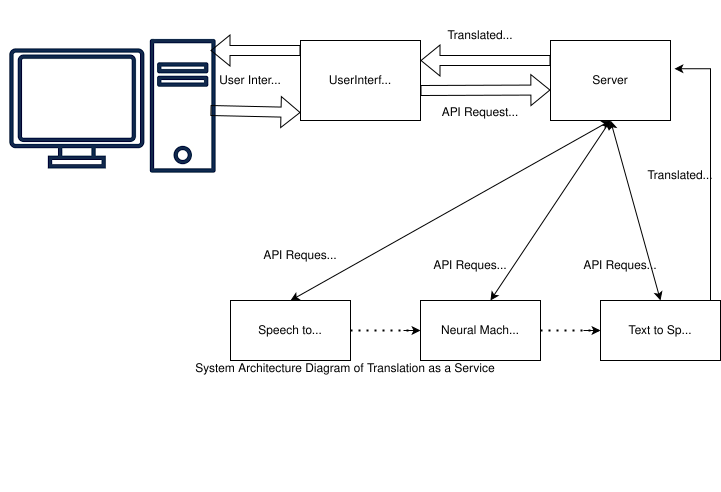
\includegraphics[height=90mm]{Images/Figures/System Architecture.png}}
  \caption{System Architecture}
  \end{center}
\end{figure}

\vspace*{0.2cm}
\newpage

\clearpage
\section{Data Flow Diagrams}
\subsection{DFD Level 0}
{\normalsize{The DFD Level 0 diagram show case the abstract view of the project, where the user shall be providing the audio source and then receive a translated audio output in the desired language.}}
\newline
\newline
\begin{figure}[h]
  \begin{center}
  \tcbox{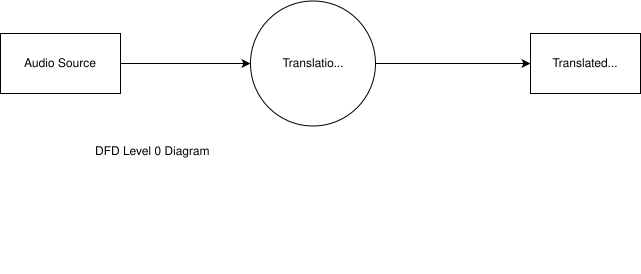
\includegraphics[height=60mm]{Images/Figures/DFD(Level 0).drawio (1) (1).png}}
  \caption{DFD Level 0}
  \end{center}
\end{figure}

\clearpage
\subsection{DFD Level 1}
{\normalsize{The Level 1 diagram, represents the module where the software resides and how the server interacts with the model for translation.}}
\newline
\newline
\begin{figure}[h]
  \begin{center}
  \tcbox{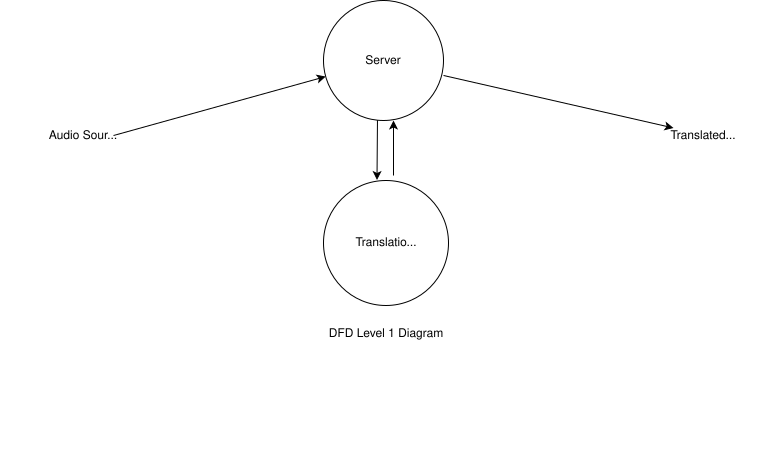
\includegraphics[height=80mm]{Images/Figures/DFD(Level 1).png}}
  \caption{DFD Level 1}
  \end{center}
\end{figure}
\newpage

\clearpage
\subsection{DFD Level 2}
{\normalsize{The DFD Level 2 represents each module present at the server and how the data is being processed from one to another. It has three models, the speech to text synthesizer, the translator, and the text to speech synthesizer.}}
\newline
\newline
\begin{figure}[h]
  \begin{center}
\tcbox{  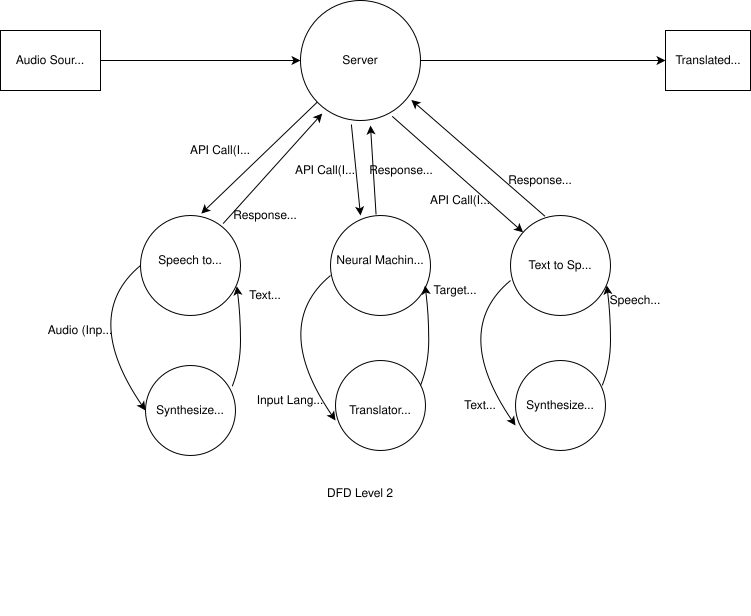
\includegraphics[height=100mm]{Images/Figures/DFD(Level2) (1).png}}
  \caption{DFD Level 2}
  \end{center}
\end{figure}

\clearpage
\section{UML Diagrams}
\subsection{Use Case Diagram}
{\normalsize{The use case diagram shows how the all actors, i.e., user and system interact with each other to make the translation successful.
\newline
The user request through the user interface by providing the appropriate input data, audio source. The server is sent a. API request for the translation. The server initiates the required sequences, and checking all the interaction and transmissions are working appropriately. The system provides the services to carry out the translation.
}}
\newline
\newline
\begin{figure}[h]
  \begin{center}
  \tcbox{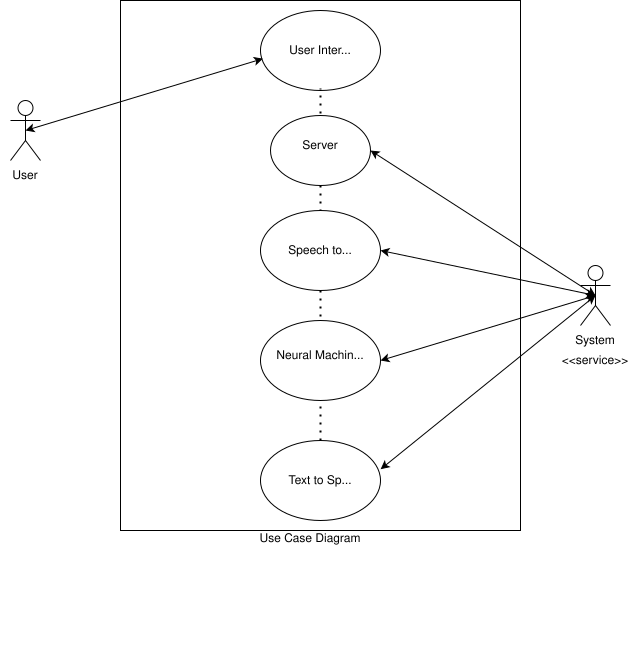
\includegraphics[height=80mm]{Images/Figures/Use Case Diagram.png}}
  \caption{Use Case Diagram}
  \end{center}
\end{figure}

\clearpage
\subsection{Activity Diagram}
{\normalsize{The activity diagram show case all the activities that occur from initialing the sever with the deployed model, to the successful interaction and translation of the audio into the desired language.
\\
In this first the server is initiated with the model deployed in it, and it checks for the status of the server. If the status is in working state, then further actions are proceeded. Otherwise, it checks for the status until it gets activated. Then the server listens for the request for services.
\\
The user starts the application section, and the connection with the server is established, for the further services. After that the user send the input data, i.e., the audio file, along with the current language and the desired language names. \\
The server then listens to the requests and check if it is a valid request and the inputs are in appropriate format. If it is valid request then further processing is done. Otherwise, error message is displayed and the server again listens for the request and data. \\
The server then transmits the request to the three models sequentially, along with checks for any error. At each stage the data is processed and transformed in the desired format.\\
Finally, if all the stages proceed without any error, then the audio file is provided as output the user, in the desired language. \\ 
The request session interaction goes on until, the user terminates the session. \\ 
}}
\newline
\newline
\begin{figure}[h]
  \begin{center}
 \tcbox{ 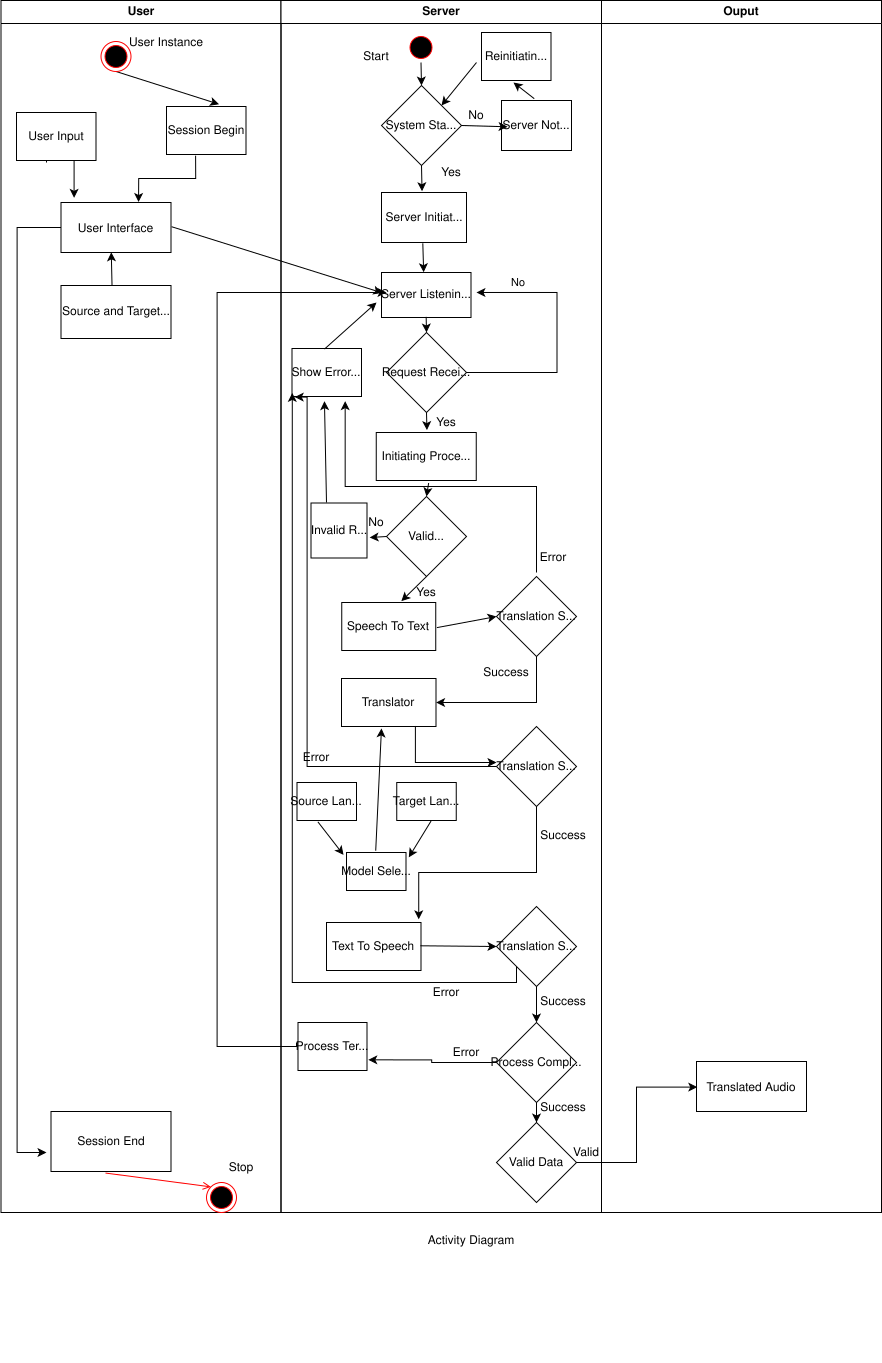
\includegraphics[height=210mm]{Images/Figures/Activity Diagram.png}}
  \caption{Activity Diagram}
  \end{center}
\end{figure}


\clearpage
\subsection{Sequence Diagram}
{\normalsize{Sequence diagram show the interaction of the user and the server, along with the session duration and all the actions that occur between them. \\ 
The session request to the server last from sending the input data to server for processing to the translated output received at the user end. \\
}}
\newline
\begin{figure}[h]
  \begin{center}
  \tcbox{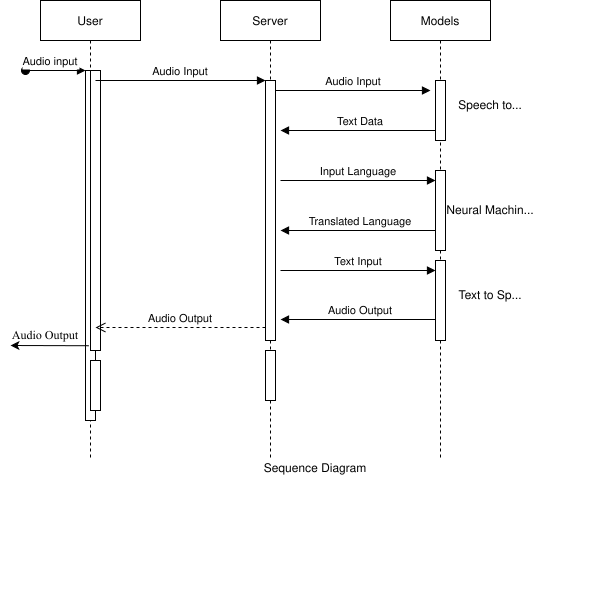
\includegraphics[height=120mm]{Images/Figures/Sequence Diagram1.png}}
  \caption{Sequence Diagram}
  \end{center}
\end{figure}

\clearpage
\subsection{Class Diagram}
\newline
\begin{figure}[h]
  \begin{center}
  \tcbox{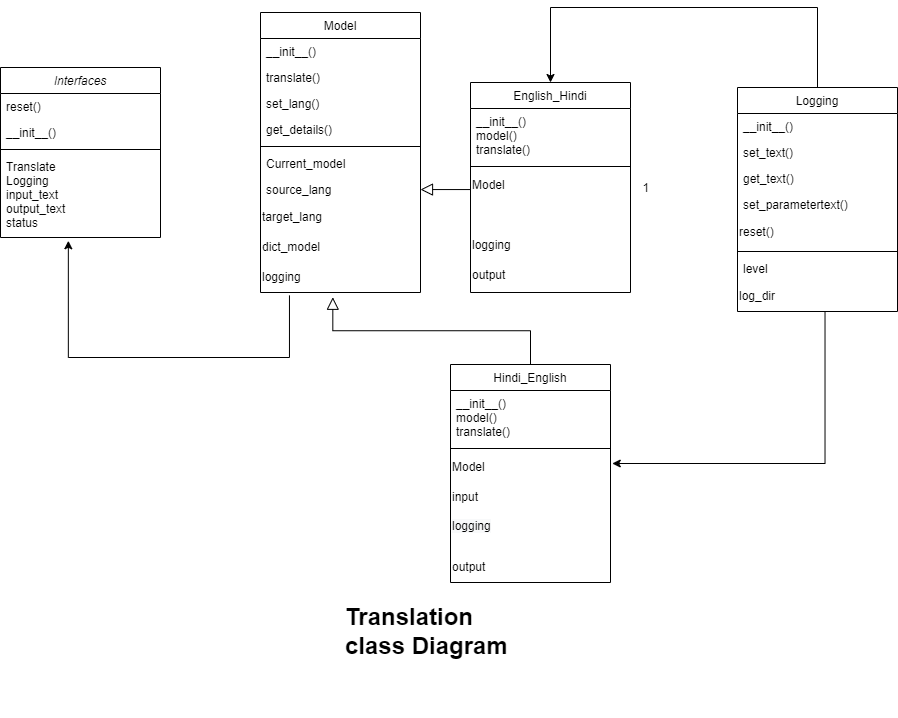
\includegraphics[height=120mm]{Images/Figures/Class_Diagram.png}}
  \caption{Class Diagram}
  \end{center}
\end{figure}

\clearpage
\chapter{Other Specifications}
\clearpage
\subsection{Advantages}
\begin{itemize}
    \item Provides an efficient way to translate one language speech to required language speech
    \item Allows you to communicate with a wide range of employees with different languages for better results. \\
\end{itemize}

\subsection{Limitations or Challenges}
\begin{itemize}
    \item Assigning weight for extracted text 
    \item Latency of the model
    \item Accuracy of the result in other language \\
\end{itemize}


\subsection{Applications}
\begin{itemize}
    \item During office meetings
    \item For communicating with different people \\
\end{itemize}
\clearpage
\chapter{Summary}
{\normalsize{\par This report studied papers. The highlights of the papers and observations are reported in chapter 2. The gap has been analyzed, based on which problem statement is designed along with its objectives. The detailed plan of all the activities is mentioned in section 1.5. \\
\par This report addresses the problems of companies with employees from different countries for their communication. Given an input, with speech, the goal is to extract text out of it, then translate the text to the desired language and give back the audio file for the required language. The accuracy of the individual components of our design is good, however, with a huge score for improvement.	
}}

\clearpage
\chapter{References}
\begin{thebibliography}{9}
\bibitem{paper1}
 Attention Is All You Need -  Ashish Vaswani∗ Google Brain avaswani@google.com Noam Shazeer∗ Google Brain noam@google.com Niki Parmar∗ Google Research nikip@google.com}
\bibitem{paper2}
Google’s Neural Machine Translation System: Bridging the Gap between Human and Machine Translation - Yonghui Wu, Mike Schuster, Zhifeng Chen, Quoc V. Le, Mohammad Norouzi yonghui,schuster,zhifengc,qvl,mnorouzi@google.com}

\bibitem{paper3}
H. Sun, R. Wang, K. Chen, M. Utiyama, E. Sumita, and T. Zhao, “Unsupervised bilingual word embedding agreement for unsupervised neural machine translation,” in Proc. 57th Annu. Meeting Assoc. Comput. Linguistics, Florence, Italy, Jul. 2019, pp. 1235–1245. 
    [2] T. Mikolov, Q. V. Le, and I. Sutskever, “Exploiting similarities among languages for machine translation,” 2013, arXiv:1309.4168
\newpage 
\bibitem{paper4}
Haque A U, Mandal P, Meng J, et al. Wind speed forecast model for wind farm based on a hybrid machine learning algorithm[J]. International Journal of Sustainable Energy, 2015, 34(1): 38- 51. 
    [2] Bahar P, Alkhouli T, Peter J T, et al. Empirical investigation of optimization algorithms in neural machine translation[J]. The Prague Bulletin of Mathematical Linguistics, 2017, 108(1): 13- 25

\end{thebibliography}
\begin{refrences}

\end{document}